\documentclass[12pt]{article}

% --------- Path definitions
\def\tikzPath{./tikz}
\def\figPath{./figures}
\def\utilPath{./utilities}

% --------- Must be set to corresponding Manuals/Bibliography directory in official FDS installation path
\def\bibPath{/Volumes/FettesBrot/GIT/github/FDS/00_Orig/Manuals/Bibliography}

\input{\bibPath/commoncommands}
\newcommand{\scarc}{{\sc ScaRC}}
\newcommand{\scarctwolevel}{{\sc ScaRC}-twolevel}
\newcommand{\scarccg}{{\sc ScaRC}-cg}
\newcommand{\scarccggmg}{{\sc ScaRC}-cggmg}
\newcommand{\scarcmultigrid}{{\sc ScaRC}-multigrid}
\newcommand{\scarcdefault}{{\sc ScaRC}-default}
\newcommand{\scarctight}{{\sc ScaRC}-tight}

\newcommand{\fftdefault}{FFT-default}
\newcommand{\ffttight}{FFT-tight}

\newcommand{\glmat}{{GLMAT}}
\newcommand{\uglmat}{{UGLMAT}}

\newcommand{\uscarc}{{\sc UScaRC}}
\newcommand{\uscarccg}{{\sc UScaRC}-cg}
\newcommand{\uscarcgmg}{{\sc UScaRC}-gmg}

\newcommand{\ols}{{1-level-Schwarz}}
\newcommand{\tls}{{2-level-Schwarz}}
\newcommand{\hone}{{hybrid\,I}}
\newcommand{\htwo}{{hybrid\,II}}

\newcommand{\ru}{\rule[-2mm]{0mm}{6mm}}
\def\restrict#1#2{{#1}\raisebox{-1.3ex}{$\,\rule{0.5pt}{3ex}\,\scriptstyle #2$}}


% --------- Packages
\usepackage{ulem}
\usepackage{amsmath,amssymb}
\usepackage{float}
\usepackage{xcolor}
\usepackage[12pt]{moresize}
\usepackage{tikz,tikz-3dplot,graphicx,mathtools}
\usetikzlibrary{positioning}
\usetikzlibrary{calc}
\usetikzlibrary{arrows}
\usetikzlibrary{arrows.meta} 
\tikzset{>=latex}

\newenvironment{myfont}{\fontfamily{\ttdefault}\selectfont}{\par}

\newcommand*\circled[1]{\tikz[baseline=(char.base)]{
            \node[shape=circle,draw,inner sep=0.2pt] (char) {#1};}}
            
\newcommand*\suci[1]{\raisebox{.5pt}{\circled{\raisebox{-.1pt} {\footnotesize {#1}}}}}

%\newcommand{\mymk}[1]{%
%   \tikz[baseline=(char.base)]\node[anchor=south west, draw,rectangle, rounded corners, inner sep=1pt, minimum size=5mm, text height=1mm](char){\raisebox{-5pt}{\ensuremath{{#1}}} ;}
\setlength{\fboxsep}{2pt}

\newcommand*\HS{{H'\,}}
\newcommand*\HSK[1]{\HS^{#1}}
\newcommand*\pH{\partial {H}}
\newcommand*\pHS{\partial {\HS}}
\newcommand*\pHSK[1]{\partial {\HS}^{#1}}
\newcommand*\HSPT{\partial^2 {\HS}}

\newcommand*\HLB[3]{\HS_{#1}^{\fbox{\raisebox{1pt}{\scriptsize{#2}}}\,,\,{#3}}} 
\newcommand*\HL[3]{\HS_{#1}^{\circled{\raisebox{-0.1pt}{\scriptsize{#2}}}\,,\,{#3}}} 
\newcommand*\HLN[2]{\HS_{#1}^{\circled{\raisebox{-0.1pt}{\scriptsize{#2}}}}} 

\newcommand*\HP[2]{\pHS^{\circled{\raisebox{-0.1pt}{\scriptsize{#1}}}\,,\,{#2}} } 
\newcommand*\HPT[2]{\HSPT^{\circled{\raisebox{0.1pt}{\scriptsize{#1}}}\,,\,{#2}}} 

\newcommand*\HPN[1]{\pHS^{\circled{\raisebox{-0.1pt}{\scriptsize{#1}}}} } 
\newcommand*\HPNT[1]{\HSPT^{\circled{\raisebox{0.1pt}{\scriptsize{#1}}}}} 

\newcommand*\HLO[2]{\overline{\HS}_{#1}^{\;{#2}}}

\newcommand*\HBO[1]{\overline{\HS}_{#1}}



\newcommand*\UIK[1]{u_i^{*,{#1}}}
\newcommand*\FIB{F_i^n  \bigg|_{\partial B}}
\newcommand*\UIB{u_i^n  \bigg|_{\partial B}}
\newcommand*\UIKB[1]{u_i^{*,{#1}} \bigg|_{\partial B}}

\newcommand*\dB{\bigg|_{\partial B}}
\newcommand*\DX{\Delta \, x}
\newcommand*\DXT{\DX^2}
\newcommand*\DXP{\partial x}
\newcommand*\DXPT{\partial x^2}
\newcommand*\DXH{\frac{\DX}{2}}

\newcommand*\DY{\Delta \, y}
\newcommand*\DYT{\DY^2}
\newcommand*\DYH{\frac{\DY}{2}}
\newcommand*\DYP{\partial y}
\newcommand*\DYPT{\partial y^2}

\newcommand*\PA{\partial}
\newcommand*\PAT{\partial^2}

\newcommand*\pD{\partial D}
\newcommand*\pM{\partial M}
\newcommand*\pB{\partial B}
\newcommand*\pxi{\partial x_i}
\newcommand*\Fin{F_i^n}


\begin{document}

%\section{McKenney-Greengard-Mayo method}

%The momentum equation in FDS can be written as 
%\[
%u_i^{n+1} = u_i^n - \Delta t \left[ F_i^n + \frac{\HSO^n}{\pxi} + \frac{\partial \HS^n}{\pxi} \right] 
%\]

\section{Basic MGM algorithm}

% --------------------------------------------------------------------------------------------------------------------------------------------
%  Predictor
% --------------------------------------------------------------------------------------------------------------------------------------------


\begin{enumerate}

\item Solve structured inhomogeneous Poisson for $H$ on $D+B$ with BC's from original problem
\[
\frac{\partial^2 H}{\pxi \pxi}  =  \frac{\partial F_i^n}{\pxi} - \left[   \frac{(\nabla \cdot \bu)	^{n+1} - (\nabla \cdot \bu)^{n} }{\Delta t} \right]  \qquad \mbox{on} \;\;D+B 
\]

\item Project velocity on $D+B$  
\[ u_i^{*,0} = u_i^n - \Delta t \left[ F_i^n + \frac{\pH}{\pxi} \right]  \qquad \mbox{on} \;\;D+B  \]

\item While error in Poisson on $D$ do for $k=0, 1, \cdots, K_{max}$

\begin{enumerate}
\item Determine BC's for ${\HSK{k}}$ 
\begin{align} 
\HSK{k}                             & = 0                                            &\mbox{on \;}  &\pD \mbox{\;(pressure BC)} \nonumber \\
\frac{\HSK{k} }{\pxi}           & = 0                                            &\mbox{on \;}  &\pD \mbox{\;(velocity BC)}.  \nonumber \\
\HSK{k}                             & = {\begin{cases} 
                                                0                & \mbox{ if } k=0 \\
                                              \HLO{}{k-1}  & \mbox{ if } k>0  \mbox{\;(simple mean BC)}  \nonumber \\ %\label{BC_Laplace} \\
                                            \end{cases} }                           &\mbox{on \;}  \pM \\
\frac{\partial {\HSK{k} }}{\pxi} &= \frac{u_i^{*,k} - 0}{\Delta t}  &\mbox{on \;} &\pB  \nonumber
\end{align}

\item Solve unstructured homogeneous Laplace for $\HSK{k}$ on $D$ with BC's from 3.(a) % (\ref{BC_Laplace})
\[   \frac{\partial^2 \HSK{k} }{\pxi \pxi} = 0 \qquad \mbox{on} \;\; D\]

\item Project velocity on $D$
\[   \UIK{k+1} =  u_i^{*,k} - \Delta t \left[\frac{\partial \HSK{k}}{\pxi} \right]  \qquad \mbox{on} \;\;D  \]

\end{enumerate}
\item Define new pressure solution $H^n := H + \HSK{k}$
\end{enumerate}

\newpage


\begin{align}
\UIK{0} & = u_i^n - \Delta t \left[ F_i^n + \frac{\pH}{\pxi} \right]     \nonumber \\
\UIK{1} & = u_i^n - \Delta t \left[ F_i^n + \frac{\pH}{\pxi} \right] - \Delta t \frac{\pHSK{0}}{\pxi}      \nonumber \\
\UIK{2} & = u_i^n - \Delta t \left[ F_i^n + \frac{\pH}{\pxi} \right] - \Delta t  \frac{\pHSK{0}}{\pxi} - \Delta t  \frac{\pHSK{1}}{\pxi}     \nonumber \\
 \end{align}

\subsection{Consider First Laplace iteration}

\begin{align}  
%
\UIK{1}\dB  &=  \underbrace{\left(u_i^n - \Delta t \left[ F_i^n + \frac{\pH}{\pxi}\right] \right) }_{u_i^{*,0}}\dB -   \Delta t \underbrace{\left( \frac{\pHSK{0}}{\pxi}\right)\dB}_{\frac{u_i^{*,0}}{\Delta t}}   = 0 \nonumber \\[2ex]
%
\UIK{1}\dM  &=  \underbrace{\left(u_i^n - \Delta t \left[ F_i^n + \frac{\pH}{\pxi}\right] \right) }_{u_i^{*,0}}\dB -   \Delta t \underbrace{\left( \frac{\pHSK{0}}{\pxi}\right)\dB}_{\frac{u_i^{*,0}}{\Delta t}}   = 0 \nonumber \\[2ex]
 \end{align}







\section{Internal boundary conditions for MGM correction step}

%\subsection{Zero boundary ("BC-0")} 

%\[  \HL{I}{1}{n} = \HL{I}{2}{n} = 0 \]
Below, I will list three different ways to define Dirichlet boundary values for $\HS$ along mesh interfaces.
To this end, let me introduce the following notation for the mean value of $\HS$ in a given node $I$  
at interface $\partial M$ in time step $t_n$, which is only related to the x-direction and the 2-mesh case in Figure (3) of your summary,
\begin{equation}
\label{BC-MEAN}
\HLO{I}{n}:=  \frac{1}{2} \left[  \HL{IBAR}{1}{n}  +  \HL{1}{2}{n} \right] 
\end{equation}


\subsection{Simple mean value (SM)} 
In your section '(6.1) A simple solution'  you proposed to use the mean values of the $\HS$ values  from the last time step $t_{n-1}$
along the interface $\partial M$

\begin{equation}
\label{BC-SM}
\HL{I}{1}{n} = \HL{I}{2}{n} = \HLO{I}{n-1}  
\end{equation}

\subsection{Linear Extrapolation (LE)}

Due to my opinion another possible approach which probably gives a little more accuracy could be to use the mean values 
$\HLO{I}{n-1}$ and $\HLO{I}{n-2}$ of the two preceding time steps $t_{n-1}$ and $t_{n-2}$
and use linear extrapolation of these two values in time 
\begin{equation}
\label{BC-LE}
\HL{I}{1}{n} = \HL{I}{2}{n} =  2 \,\HLO{I}{n-1} - \, \HLO{I}{n-2}
\end{equation}
  
Of course it is the question of initial values for this extrapolation. I started with it only after the 2nd time-step and took (SM) before. 
But also for (SM) there is the question of the proper initial values from my point of view. Currently, I simply use zero as initial values $\HS$ values for $t_0$. However, I could also imagine to take a little more effort here (but more about this later).

\subsection{Taylor Series (TS)}

Now, let's come to your '(6.2) Complex solution' based on a Taylor series expansion.
\begin{align}
\HL{IBAR}{1}{n}  & =  \HL{I}{1}{n} - \frac{1}{1!}\frac{\DX}{2} \frac{\HPN{1}} {\DXP} \bigg|_{I}^n 
                                                    + \frac{1}{2!}\left(\frac{\DX}{2}\right)^2 \frac{\HPNT{1}} {\DXPT} \bigg|_{I}^n  - \cdots \label{BC-TSA}
 \\[1ex]
\HL{1}{2}{n}  & =  \HL{I}{2}{n} + \frac{1}{1!}\frac{\DX}{2} \frac{\HPN{2}} {\DXP} \bigg|_{I}^n 
                                                    + \frac{1}{2!}\left(\frac{\DX}{2}\right)^2 \frac{\HPNT{2}} {\DXPT} \bigg|_{I}^n  + \cdots   \nonumber                                                         
\end{align}
or shorter
\begin{align}
\HL{IBAR}{1}{n}  & =  \HL{I}{1}{n} - \frac{\DX}{2} \frac{\HPN{1}} {\DXP} \bigg|_{I}^n 
                                                     + \frac{\DXT}{\color{red}{8}} \frac{\HPNT{1}} {\DXPT} \bigg|_{I}^n  - \cdots \label{BC-TSB}
 \\[1ex]
\HL{1}{2}{n}  & =  \HL{I}{2}{n} + \frac{\DX}{2} \frac{\HPN{2}} {\DXP} \bigg|_{I}^n 
                                                     + \frac{\DXT}{\color{red}{8}}\frac{\HPNT{2}} {\DXPT} \bigg|_{I}^n  + \cdots    \nonumber                                                 
\end{align}



%Please have a look at the '8' in the denominator where you had a '4'. But we still have to divide the $(\DX / 2)^2$ term by '$2!$'. Isn't that correct? 
For the ghost cell values $\HL{IBAR+1}{1}{n}$ and $\HL{0}{2}{n}$ we consider linear extrapolation
\begin{align}
\label{Extrapolation}
\HL{{\color{red}{IBAR+1}}}{1}{n} & = 2\, \HL{{\color{green}{I}}}{1}{n} -  \HL{{\color{red}{IBAR}}}{1}{n} \\[1ex]
\HL{{\color{blue}{0}}}{2}{n} & = 2 \,\HL{{\color{green}{I}}}{2}{n} -  \HL{{\color{blue}{1}}}{2}{n}   \nonumber     
\end{align}

\begin{figure}[H]
\begin{center}
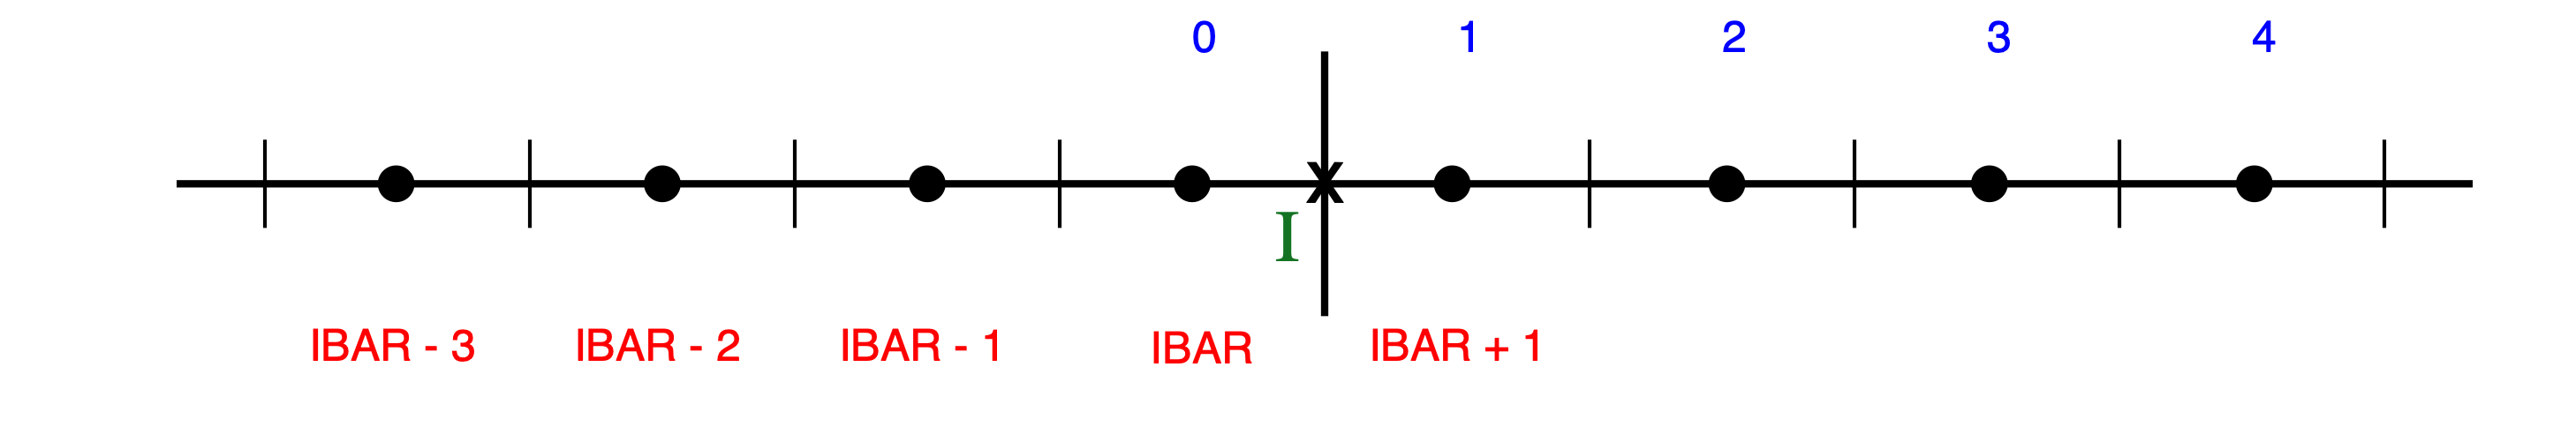
\includegraphics[width=14cm]{\figPath/DecompositionX.png}
\end{center}
\caption{Decomposition in x-direction}
\label{FIG_DecompositionX}
\end{figure}
In the following I will list the individual steps in great detail to avoid sign errors or similar in a possible implementation. 
First of all the following simple transformation is done based on (\ref{BC-TSB})


\begin{align}
\label{BC-TSB}
\HL{I}{1}{n} & = \HL{IBAR}{1}{n}  + \frac{\DX}{2} \frac{\HPN{1}} {\DXP} \bigg|_{I}^n 
                                                      - \frac{\DXT}{8} \frac{\HPNT{1}} {\DXPT} \bigg|_{I}^n  + \cdots  \\[1ex]
\HL{I}{2}{n} & =  \HL{1}{2}{n}  - \frac{\DX}{2} \frac{\HPN{2}} {\DXP} \bigg|_{I}^n 
                                                - \frac{\DXT}{8}\frac{\HPNT{2}} {\DXPT} \bigg|_{I}^n  - \cdots         \nonumber                                            
\end{align}


Now, substituting the interface values (\ref{BC-TSB}) into the extrapolation settings (\ref{Extrapolation}) in order to eliminate them
\begin{align}
\HL{IBAR+1}{1}{n} & \; \approx 2 \cdot \left( \HL{IBAR}{1}{n}  + \frac{\DX}{2} \frac{\HPN{1}} {\DXP} \bigg|_{I}^n 
                                                      - \frac{\DXT}{8} \frac{\HPNT{1}} {\DXPT} \bigg|_{I}^n  \right) -  \HL{IBAR}{1}{n} \label{BC-TSD}
 \\[1ex]
\HL{0}{2}{n} & \approx \; 2 \cdot \left( \HL{1}{2}{n}  - \frac{\DX}{2} \frac{\HPN{2}} {\DXP} \bigg|_{I}^n 
                                                - \frac{\DXT}{8}\frac{\HPNT{2}} {\DXPT} \bigg|_{I}^n \right)    -  \HL{1}{2}{n}      \nonumber                                           
\end{align}
which finally leads to

\begin{align}
\HL{IBAR+1}{1}{n} & \approx \;  \HL{IBAR}{1}{n}  + \DX \frac{\HPN{1}} {\DXP} \bigg|_{I}^n 
                                                      - \frac{\DXT}{4} \frac{\HPNT{1}} {\DXPT} \bigg|_{I}^n  \label{BC-TSD}
 \\[1ex]
\HL{0}{2}{n} & \approx  \HL{1}{2}{n}  - \DX \frac{\HPN{2}} {\DXP} \bigg|_{I}^n 
                                                - \frac{\DXT}{4}\frac{\HPNT{2}} {\DXPT} \bigg|_{I}^n     \nonumber                                           
\end{align}

\newpage
\subsubsection{The second derivative}
As you wrote, the second derivative in x must be the negative of the second derivative in y, because we solve the Laplace problem.
%\[ \frac{\HPNT{1}}{\DXPT} \bigg|_{I}^n  = -  \frac{\HPNT{1}}{\DYPT}\bigg|_{I}^n   \]

But concerning your second step in the derivation under '(6.3) Second derivative' I am confused right now. There you use two terms, first a difference quotient in y and then one in x (but our goal is to replace '$IBAR+1$'). Here, I suppose we only need the first one in y such that finally holds
\begin{align}
\label{BC-TSE}
 \frac{\HPNT{1}}{\DXPT} \bigg|_{I}^n  & = -  \frac{\HPNT{1}}{\DYPT}\bigg|_{I}^n   \approx 
                                                                  - \,\frac{\HL{IBAR,j-1}{1}{n} - 2 \HL{IBAR,j}{1}{n} + \HL{IBAR,j+1}{1}{n}}{\DYT}        \\                                                                 
 \frac{\HPNT{2}}{\DXPT} \bigg|_{I}^n  & = -  \frac{\HPNT{2}}{\DYPT}\bigg|_{I}^n   \approx 
                                                                  - \, \frac{\HL{1,j-1}{2}{n} - 2 \HL{1,j}{2}{n} + \HL{1,j+1}{2}{n}}{\DYT} 
\end{align}                                                                  

What do you think about this? This term adds matrix entries in y-direction.

\subsubsection{The first derivative}
For the sake of completeness I also list your steps to define the first derivation. Based on the previous solutions
$\HL{\,}{1}{n-1}$ and $\HL{\,}{2}{n-1}$, we approximate the derivative on the mesh interface by

\[ \frac {\HPNT{1}}{\DXP}\bigg|_{I}^n  = \frac {\HPNT{2}}{\DXP}\bigg|_{I}^n \approx \frac{\HL{1}{2}{n-1} - \HL{IBAR}{1}{n-1}} {\DX}\]

\subsubsection{Putting everything together}

Now, inserting all this stuff into (\ref{BC-TSD}) we get
\begin{align}
\label{BC-TSF}
\HL{IBAR+1,j}{1}{n} & \approx \;  \HL{IBAR,j}{1}{n}  + \DX \left( \frac{\HL{1}{2}{n-1} - \HL{IBAR,j}{1}{n-1}} {\DX}\right)
                                                      - \frac{\DXT}{4}   \left(-\,\frac{\HL{IBAR,j-1}{1}{n} - 2 \HL{IBAR,j}{1}{n} + \HL{IBAR,j+1}{1}{n}}{\DYT} \right)
 \\[1ex]
\HL{0,j}{2}{n} & \approx  \HL{1,j}{2}{n}  - \DX \left(\frac{\HL{1,j}{2}{n-1} - \HL{IBAR,j}{1}{n-1}} {\DX}\right)
                                                - \frac{\DXT}{4} \left(-\,\frac{\HL{1,j-1}{2}{n} - 2 \HL{1,j}{2}{n} + \HL{1,j+1}{2}{n}}{\DYT}  \right)    \nonumber                                           
\end{align}

And if I didn't make a mistake somewhere (which is not unlikely in this mess), this finally leads to
\begin{align}
\label{BC-TSF}
\HL{IBAR+1,j}{1}{n} & \approx \;  \HL{IBAR,j}{1}{n}  + \left(\HL{1,j}{2}{n-1} - \HL{IBAR,j}{1}{n-1}\right) 
                                                + \frac{\DXT}{4\DYT}   \left(\HL{IBAR,j-1}{1}{n} - 2 \HL{IBAR,j}{1}{n} + \HL{IBAR,j+1}{1}{n} \right) \\[1ex]
\HL{0,j}{2}{n} & \approx  \HL{1,j}{2}{n}  - \left( \HL{1,j}{2}{n-1} - \HL{IBAR,j}{1}{n-1}\right)
                                                + \frac{\DXT}{4\DYT}   \left(\HL{1,j-1}{2}{n} - 2 \HL{1,j}{2}{n} + \HL{1,j+1}{2}{n}\right)      \nonumber                                           
\end{align}
When using these terms in the matrix stencil for cells adjacent to the mesh interface, the previous '${n-1}$' terms add up to the right hand side and the current '$n$' terms to the matrix itself.

\subsubsection{Substituting the ghost values in the matrix stencil in 2D}
%
\paragraph{Mesh 1:} 
For a cell in mesh 1 adjacent to the mesh interface the usual Laplace matrix stencil is
\[   \frac{ \HL{IBAR-1,j}{1}{n} -2 \HL{IBAR,j}{1}{n} + \HL{IBAR+1,j}{1}{n} }{\DXT} +  
    \frac{ \HL{IBAR,j-1}{1}{n} -2 \HL{IBAR,j}{1}{n} + \HL{IBAR,j+1}{1}{n} }{\DYT} = 0 \]
Now, substituting the '$IBAR+1$' component based on the derivation in (\ref{BC-TSF}), we get 
\[ {\scriptstyle  \frac{ \HL{IBAR-1,j}{1}{n} -2 \HL{IBAR,j}{1}{n} 
+ \left[ \HL{IBAR,j}{1}{n}  + \left(\HL{1,j}{2}{n-1} - \HL{IBAR,j}{1}{n-1}\right) + \frac{\DXT}{4\DYT}   \left(\HL{IBAR,j-1}{1}{n} - 2 \HL{IBAR,j}{1}{n} + \HL{IBAR,j+1}{1}{n} \right) \right]}{\DXT}
+      \frac{ \HL{IBAR,j-1}{1}{n} -2 \HL{IBAR,j}{1}{n} + \HL{IBAR,j+1}{1}{n} }{\DYT} = 0}
\]
Let's first move the previous '${n-1}$' terms on the right hand side and sum up the obvious
\[ {\scriptstyle  \frac{ \HL{IBAR-1,j}{1}{n} - \HL{IBAR,j}{1}{n}   
+ \frac{\DXT}{4\DYT}   \left(\HL{IBAR,j-1}{1}{n} - 2 \HL{IBAR,j}{1}{n} + \HL{IBAR,j+1}{1}{n} \right) }{\DXT}
+      \frac{ \HL{IBAR,j-1}{1}{n} -2 \HL{IBAR,j}{1}{n} + \HL{IBAR,j+1}{1}{n} }{\DYT} = -\frac{\HL{1,j}{2}{n-1} - \HL{IBAR,j}{1}{n-1}}{\DXT} }
\]
and then resort the whole stuff
\[ {\scriptstyle 
      \HL{IBAR,j-1}{1}{n} \left( \frac {1}{4\DYT} + \frac {1}{\DYT}    \right)
 +   \HL{IBAR-1,j}{1}{n} \left( \frac {1}{\DXT} \right)
 +   \HL{IBAR,j}{1}{n} \left( -\frac {1}{\DXT} - \frac {1}{2\DYT} - \frac {2}{\DYT}    \right)
 +   \HL{IBAR,j+1}{1}{n} \left( \frac {1}{4\DYT}   + \frac {1}{\DYT}    \right)
    = -\frac{\HL{1,j}{2}{n-1} - \HL{IBAR,j}{1}{n-1}}{\DXT} }
\]
which finally gives the new matrix entries for the corresponding matrix line for cell $(IBAR,j)$ in mesh 1. 

%\HL{2,j}{2}{n}
\paragraph{Mesh 2:} 

\vspace{0.5cm}
For a cell in mesh 2 adjacent to the mesh interface the usual Laplace matrix stencil is
\[   
   \frac{ \HL{0,j}{2}{n} -2 \HL{1,j}{2}{n} + \HL{2,j}{2}{n} }{\DXT} +  
   \frac{ \HL{1,j-1}{2}{n} -2 \HL{1,j}{2}{n} + \HL{1,j+1}{2}{n} }{\DYT} = 0 
\]
Now, substituting the '$0$' component based on the derivation in (\ref{BC-TSF}), we get 
\[ 
  {\scriptstyle  
   \frac{ 
   \left[
         \HL{1,j}{2}{n}  - \left( \HL{1,j}{2}{n-1} - \HL{IBAR,j}{1}{n-1}\right)
      + \frac{\DXT}{4\DYT}   \left(\HL{1,j-1}{2}{n} - 2 \HL{1,j}{2}{n} + \HL{1,j+1}{2}{n}\right)
   \right] 
   -2 \HL{1,j}{2}{n} + \HL{2,j}{2}{n} }{\DXT} +  
   \frac{ \HL{1,j-1}{2}{n} -2 \HL{1,j}{2}{n} + \HL{1,j+1}{2}{n} }{\DYT} = 0 
   }
\]
Let's first move the previous '${n-1}$' terms on the right hand side and sum up the obvious
\[ 
  {\scriptstyle  
   \frac{ 
         -\HL{1,j}{2}{n}  
      + \frac{\DXT}{4\DYT}   \left(\HL{1,j-1}{2}{n} - 2 \HL{1,j}{2}{n} + \HL{1,j+1}{2}{n}\right)
 + \HL{2,j}{2}{n} }{\DXT} +  
   \frac{ \HL{1,j-1}{2}{n} -2 \HL{1,j}{2}{n} + \HL{1,j+1}{2}{n} }{\DYT} =  \frac{\HL{1,j}{2}{n-1} - \HL{IBAR,j}{1}{n-1}}{\DXT}
   }
\]


and then resort the whole stuff
\[ {\scriptstyle 
      \HL{1,j-1}{2}{n} \left( \frac {1}{4\DYT} + \frac {1}{\DYT}    \right)
 +   \HL{2,j}{2}{n} \left( \frac {1}{\DXT} \right)
 +   \HL{1,j}{2}{n} \left( -\frac {1}{\DXT} - \frac {1}{2\DYT} - \frac {2}{\DYT}    \right)
 +    \HL{1,j+1}{2}{n} \left( \frac {1}{4\DYT}   + \frac {1}{\DYT}    \right)
    = \frac{\HL{1,j}{2}{n-1} - \HL{1,j}{1}{n-1}}{\DXT} }
\]
which finally gives the new matrix entries for the corresponding matrix line for cell $(1,j)$ in mesh 2.

\newpage

\subsubsection{Substituting the ghost values in the matrix stencil in 3D}
%
\paragraph{Mesh 1:} 
For a cell in mesh 1 adjacent to the mesh interface the usual Laplace matrix stencil is
\begin{align}   
    & \frac{ \HL{IBAR-1,j,k}{1}{n} -2 \HL{IBAR,j,k}{1}{n} + \HL{IBAR+1,j,k}{1}{n} }{\DXT} \\
+  & \frac{ \HL{IBAR,j-1,k}{1}{n} -2 \HL{IBAR,j,k}{1}{n} + \HL{IBAR,j+1,k}{1}{n} }{\DYT} \\
+  & \frac{ \HL{IBAR,j-1,k}{1}{n} -2 \HL{IBAR,j,k}{1}{n} + \HL{IBAR,j+1,k}{1}{n} }{\DYT} \\
& \hspace{5cm}= 0 
 \end{align}
Now, substituting the '$IBAR+1$' component based on the derivation in (\ref{BC-TSF}), we get 
\[ {\scriptstyle  \frac{ \HL{IBAR-1,j}{1}{n} -2 \HL{IBAR,j}{1}{n} 
+ \left[ \HL{IBAR,j}{1}{n}  + \left(\HL{1,j}{2}{n-1} - \HL{IBAR,j}{1}{n-1}\right) + \frac{\DXT}{4\DYT}   \left(\HL{IBAR,j-1}{1}{n} - 2 \HL{IBAR,j}{1}{n} + \HL{IBAR,j+1}{1}{n} \right) \right]}{\DXT}
+      \frac{ \HL{IBAR,j-1}{1}{n} -2 \HL{IBAR,j}{1}{n} + \HL{IBAR,j+1}{1}{n} }{\DYT} = 0}
\]
Let's first move the previous '${n-1}$' terms on the right hand side and sum up the obvious
\[ {\scriptstyle  \frac{ \HL{IBAR-1,j}{1}{n} - \HL{IBAR,j}{1}{n}   
+ \frac{\DXT}{4\DYT}   \left(\HL{IBAR,j-1}{1}{n} - 2 \HL{IBAR,j}{1}{n} + \HL{IBAR,j+1}{1}{n} \right) }{\DXT}
+      \frac{ \HL{IBAR,j-1}{1}{n} -2 \HL{IBAR,j}{1}{n} + \HL{IBAR,j+1}{1}{n} }{\DYT} = -\frac{\HL{1,j}{2}{n-1} - \HL{IBAR,j}{1}{n-1}}{\DXT} }
\]
and then resort the whole stuff
\[ {\scriptstyle 
      \HL{IBAR,j-1}{1}{n} \left( \frac {1}{4\DYT} + \frac {1}{\DYT}    \right)
 +   \HL{IBAR-1,j}{1}{n} \left( \frac {1}{\DXT} \right)
 +   \HL{IBAR,j}{1}{n} \left( -\frac {1}{\DXT} - \frac {1}{2\DYT} - \frac {2}{\DYT}    \right)
 +   \HL{IBAR,j+1}{1}{n} \left( \frac {1}{4\DYT}   + \frac {1}{\DYT}    \right)
    = -\frac{\HL{1,j}{2}{n-1} - \HL{IBAR,j}{1}{n-1}}{\DXT} }
\]
which finally gives the new matrix entries for the corresponding matrix line for cell $(IBAR,j)$ in mesh 1. 


This is all done in extreme detail now, but I found it more secure than on paper, thanks to Copy\&Paste. I really hope that not one million sign and component errors have crept in here. I'll focus on the code again now.

Have I understood your suggested procedure correctly by then or do you think that the above derivations are correct so far?


\subsection{True (approximate) solution}

\begin{figure}[H]
\begin{center}
\includegraphics[width=12cm]{\figPath/mgm2.png}
\end{center}
\caption{Interface between two adjacent meshes}
\label{FIG_InterfaceTwo}
\end{figure}

Goal is to enforce $\nabla^2 \HS = 0$ on $\pM$

\[ \frac{\HBO{I-1,j} - 2 \HBO{I,j} + \HBO{I+1,j}}{\DXT}  +  \frac{\HBO{I,j-1} - 2 \HBO{I,j} + \HBO{I,j+1}}{\DYT} = 0\]

\noindent This can be transformed to

%\begin{align}  
%\frac{2 \HBO{I,j}}{\DXT}  +  \frac{2 \HBO{I,j}}{\DYT}  &=  \frac{\HBO{i-1,j} + \HBO{i+1,j}}{\DXT}  +  \frac{\HBO{i-1,j}  + \HBO{i+1,j}}{\DYT} \\[2ex]
%\frac{2 \HBO{I,j}\DYT + 2\HBO{I,j}\DXT}{\DXT\DYT}   &=  \frac{\HBO{i-1,j} + \HBO{i+1,j}}{\DXT}  +  \frac{\HBO{i-1,j}  + \HBO{i+1,j}}{\DYT} \\[2ex]
%2\left(\DXT +  \DYT\right) \HBO{I,j} &=\DXT\DYT \left( \frac{\HBO{i-1,j} + \HBO{i+1,j}}{\DXT}  +  \frac{\HBO{i-1,j}  + \HBO{i+1,j}}{\DYT}\right) \\[2ex]
%\HBO{I,j} &= \frac{\DYT\left( \HBO{i-1,j} + \HBO{i+1,j} \right) + \DXT \left(\HBO{i-1,j}  + \HBO{i+1,j} \right)}{2\left(\DXT +  \DYT\right)}
%\end{align}

\begin{align}  
%\HBO{I,j}\left[\frac{2 }{\DXT}  +  \frac{2 }{\DYT}\right]  &=  \frac{\HBO{i-1,j} + \HBO{i+1,j}}{\DXT}  +  \frac{\HBO{i-1,j}  + \HBO{i+1,j}}{\DYT} \\[2ex]
\HBO{I,j} &=  \left[\frac{\HBO{I-1,j} + \HBO{I+1,j}}{\DXT}  +  \frac{\HBO{I,j-1}  + \HBO{I,j+1}}{\DYT}\right] \biggl/ \left[\frac{2 }{\DXT}  +  \frac{2 }{\DYT}\right] \nonumber  
\end{align}
\noindent where (in the simplest case with equidistant grid size of same resolution in every mesh)

\begin{align}  
\HBO{I-1,j}  &= \frac{1}{2} (\HL{i-1,j}{1}{n-1} + \HL{i,j}{1}{n-1})  \nonumber \\[2ex]
\HBO{I+1,j} &= \frac{1}{2} (\HL{1,j}{2}{n-1} + \HL{2,j}{2}{n-1}) \nonumber \\[2ex]
\HBO{I,j-1} &= \frac{1}{2} (\HL{i,j-1}{1}{n-1} + \HL{1,j-1}{2}{n-1}) \nonumber \\[2ex]
\HBO{I,j+1} &= \frac{1}{2} (\HL{i,j+1}{1}{n-1} + \HL{1,j+1}{2}{n-1}) \label{EQ_HB_VALUES}
\end{align}  


\subsection{Interface meets external boundary}

Let's have a look to the case, where the interface meets an external boundary

\begin{figure}[H]
\begin{center}
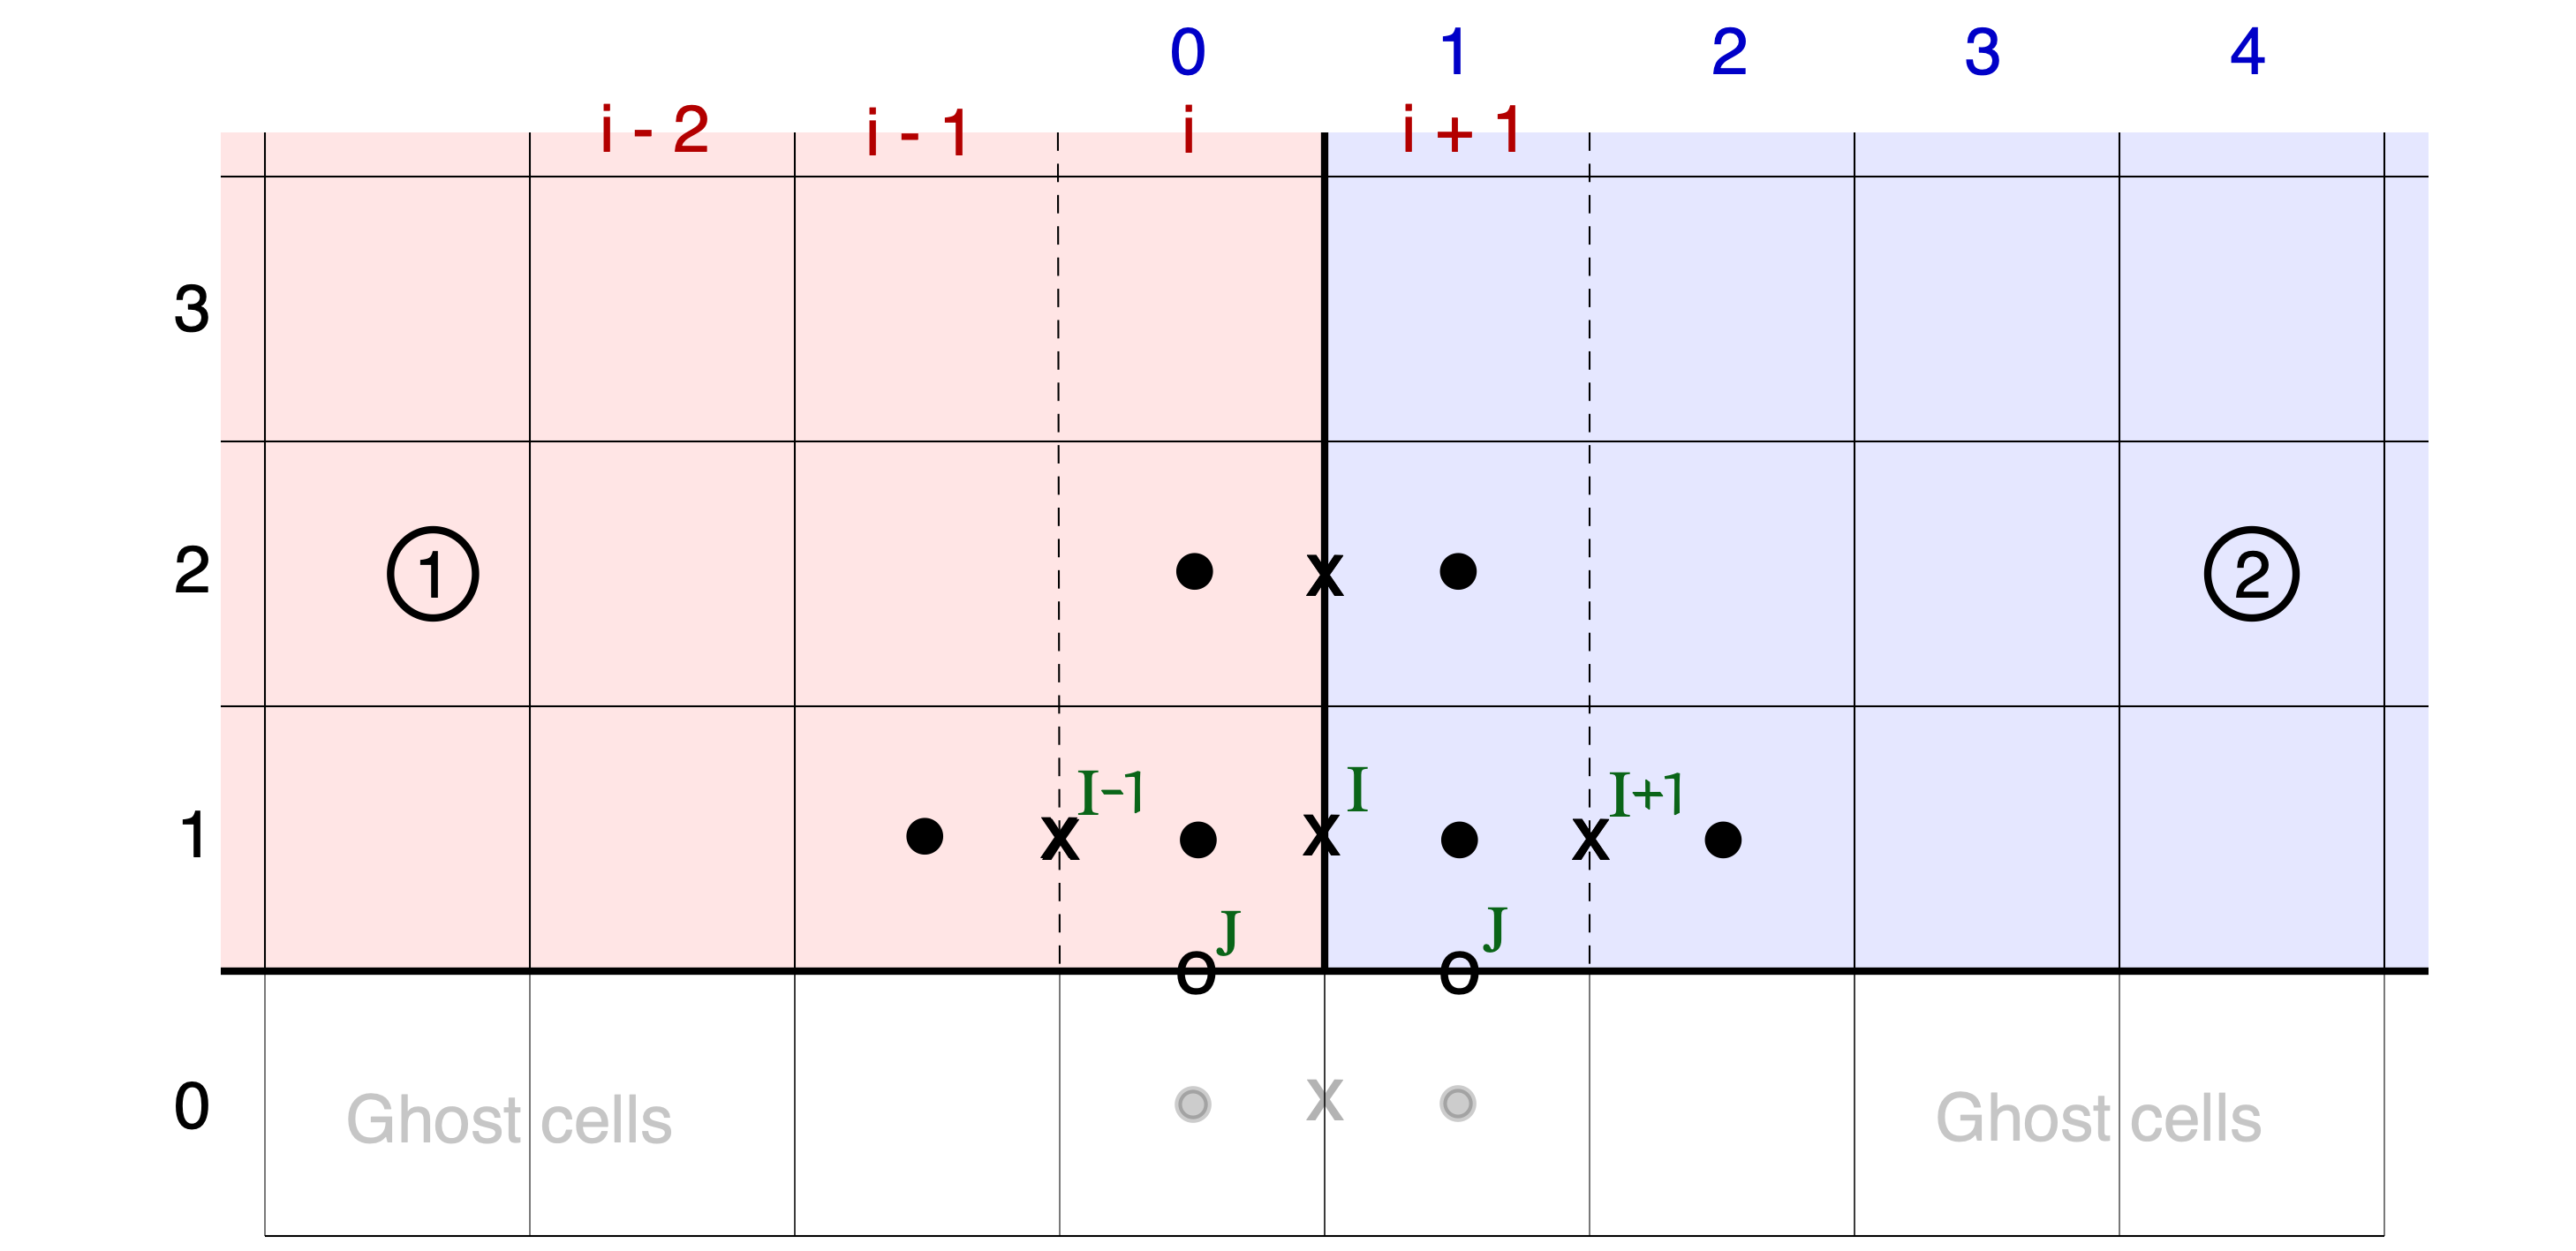
\includegraphics[width=14cm]{\figPath/MGM_Boundary.png}
\end{center}
\caption{Interface meets an external boundary}
\label{FIG_InterfaceBdry}
\end{figure}

%\noindent For the corresponding stencil in an interface node adjacent to the external boundary it holds
%\begin{align}  
%\HBO{I,1} &=  \left[\frac{\HBO{I-1,1} + \HBO{I+1,1}}{\DXT}  +  \frac{\HBO{I,0}  + \HBO{I,2}}{\DYT}\right] \biggl/ \left[\frac{2 }{\DXT}  +  \frac{2 }{\DYT}\right] \nonumber  
%\end{align}

\noindent The usual stencil in point $(I,1)$ looks like 
\[ \frac{\HBO{I-1,1} - 2 \HBO{I,1} + \HBO{I+1,1}}{\DXT}  +  \frac{\HBO{I,0} - 2 \HBO{I,1} + \HBO{I,2}}{\DYT} = 0\]


\subsubsection{Dirichlet case}

\noindent  The Dirichlet boundary values in the lower $y$-direction are defined as
\[\HBO{I,0}  = 2 \HBO{I,J} - \HBO{I,1} \qquad \rightarrow \qquad  \HBO{I,0}  =  - \HBO{I,1} \]
\noindent because $\HBO{I,J}=0$ due to the homogeneous Laplace boundary.
\noindent Thus, the stencil in $\HBO{I,1}$ looks like
\[\frac{\HBO{I-1,1} - 2 \HBO{I,1} + \HBO{I+1,1}}{\DXT}  +  \frac{ {\color{red}{-\HBO{I,1}}} - 2 \HBO{I,1} + \HBO{I,2}}{\DYT} = 0 \]
\noindent which results in  
\[\HBO{I,1} =  \left[\frac{\HBO{I-1,1} + \HBO{I+1,1}}{\DXT}  +  \frac{\HBO{I,2}}{\DYT}\right] \biggl/ \left[\frac{2 }{\DXT}  +  \frac{3}{\DYT}\right]\]

\newpage
\subsubsection{Neumann case}

\noindent  The Neumann boundary values in the lower $y$-direction are defined as
\[\frac{\HBO{I,0} - \HBO{I,1}}{\DY}  = 0   \qquad \rightarrow \qquad   \HBO{I,0} = \HBO{I,1} \]
\noindent Thus, the stencil in $\HBO{I,1}$ looks like
\[\frac{\HBO{I-1,1} - 2 \HBO{I,1} + \HBO{I+1,1}}{\DXT}  +  \frac{ {\color{red}{\HBO{I,1}}} - 2 \HBO{I,1} + \HBO{I,2}}{\DYT} = 0 \]
\noindent which results in  
\[\HBO{I,1} =  \left[\frac{\HBO{I-1,1} + \HBO{I+1,1}}{\DXT}  +  \frac{\HBO{I,2}}{\DYT}\right] \biggl/ \left[\frac{2 }{\DXT}  +  \frac{1}{\DYT}\right]\]


\subsection{Multiple meshes meet}
\noindent We still have to think of the treatment of cases where multiple meshes meet together. Please have a look at the node in the yellow mesh 4 which is not available by the usual WALL(IW) structures on mesh 1. Here, I think, we should use an alternative treatment or exchange the related values by a global data exchange (which would be possible, but would cost this exchange).

\begin{figure}[H]
\begin{center}
\includegraphics[width=12cm]{\figPath/mgm4.png}
\end{center}
\caption{Interfaces in case of 4 adjacent meshes}
\label{FIG_InterfaceFour}
\end{figure}

\begin{align}  
\HBO{I,j} &=  \left[\frac{\HBO{I-1,j} + \HBO{I+1,j}}{\DXT}  +  \frac{\HBO{I,j-1}  + \HBO{I,j+1}}{\DYT}\right] \biggl/ \left[\frac{2 }{\DXT}  +  \frac{2 }{\DYT}\right] \nonumber  
\end{align}
\noindent with

\begin{align}  
\HBO{I-1,j}  &= \frac{1}{2} (\HL{i-1,j}{1}{n-1} + \HL{i,j}{1}{n-1})  \nonumber \\[2ex]
\HBO{I+1,j} &= \frac{1}{2} (\HL{1,j}{2}{n-1} + \HL{2,j}{2}{n-1}) \nonumber \\[2ex]
\HBO{I,j+1} &= \frac{1}{2} (\HL{i,j+1}{1}{n-1} + \HL{1,j+1}{2}{n-1}) \nonumber \\[2ex]
\HBO{I,j-1} &= \color{red} {\frac{1}{2} (\HL{i,k}{3}{n-1} + \HL{1,m}{4}{n-1})} \nonumber \\[2ex]
\end{align}  




%
\section{Test cases}

\subsection{Verification of basic MGM implementation}
The first step of my test series was to verify the basic correctness of my implementation of the MGM methodology. For this purpose I started from the requirement that for a single mesh case MGM (as an unstructured solver) should yield exactly the same solution as UGLMAT or USCARC.

In fact, I could actually prove this for many different single mesh test cases, so that I no longer doubt the correct calculation and assignment of Neumann boundary values along inner obstructions.



\subsection{Comparison of different boundary conditions along $\partial M$}
My next step was to compare UGLMAT and USCARC versus MGM for different multi-mesh cases. 
As boundary values along $\partial M$ I tested the 'Simple mean value (SM)' and the 'Linear Extrapolation (LE)'. The Taylor-variant is in development, but not yet finished.

The (LE) variant was worth a test from my point of view, because it as relatively easy to implement and storing the additionally needed interface values from the second last step '${n-2}$' does not require much space. 

\subsubsection{Case 1}
Let's start with a very simple test with only one obstruction which is completely contained in one mesh. 
\begin{figure}[H]
\begin{center}
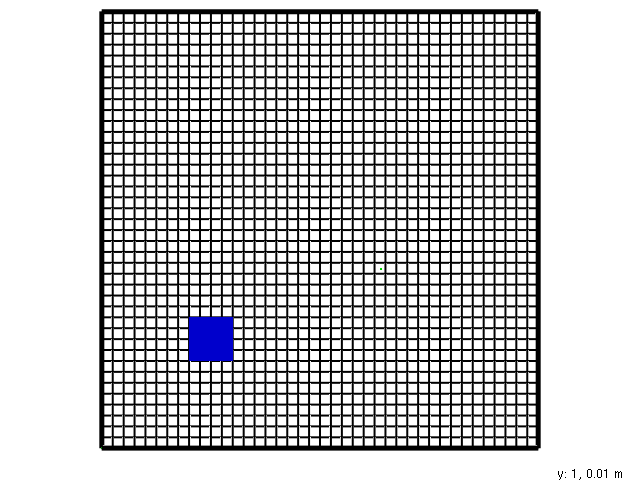
\includegraphics[width=7cm]{\figPath/b1_s0002.png}
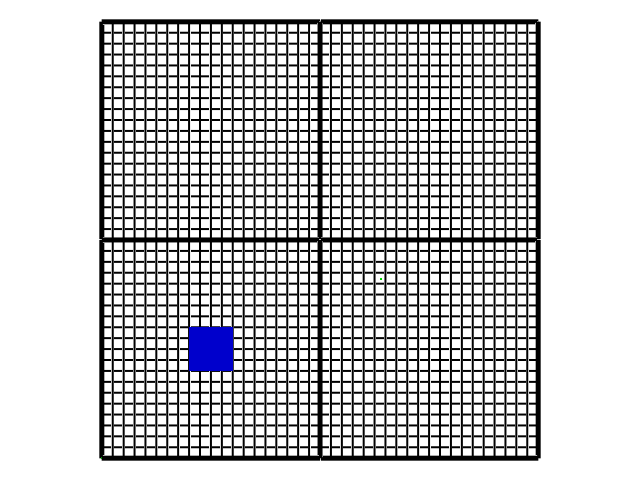
\includegraphics[width=7cm]{\figPath/b4_le_s0002.png}
\end{center}
\caption{Case 1}
\label{FIG_MGM_Grid}
\end{figure}
\newpage
Then the simple mean value (SM) gives

\begin{figure}[H]
\begin{center}
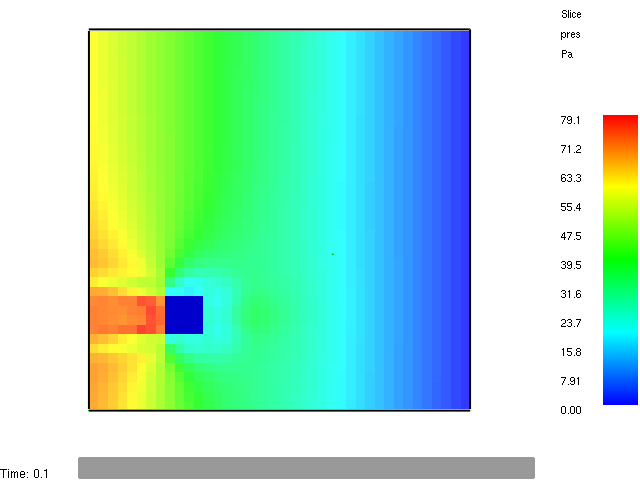
\includegraphics[width=8cm]{\figPath/b1_0062.png}
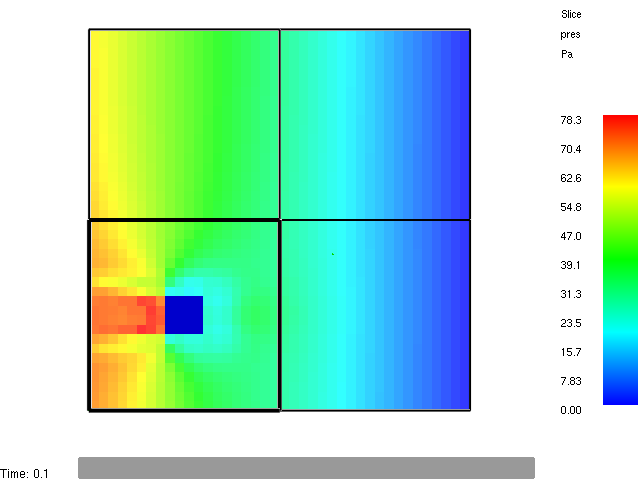
\includegraphics[width=8cm]{\figPath/b4_sm_0062.png}
\end{center}
\caption{Simple mean value  (SM) for Case 1}
\label{FIG_MGM_Grid}
\end{figure}


and the linear extrapolation setting (LE) gives

\begin{figure}[H]
\begin{center}
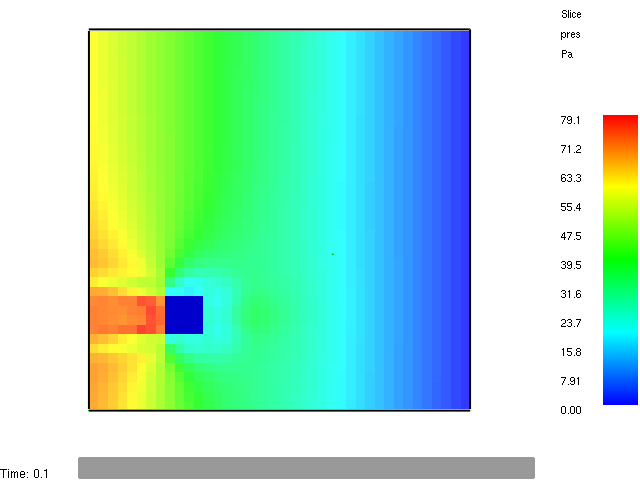
\includegraphics[width=8cm]{\figPath/b1_0062.png}
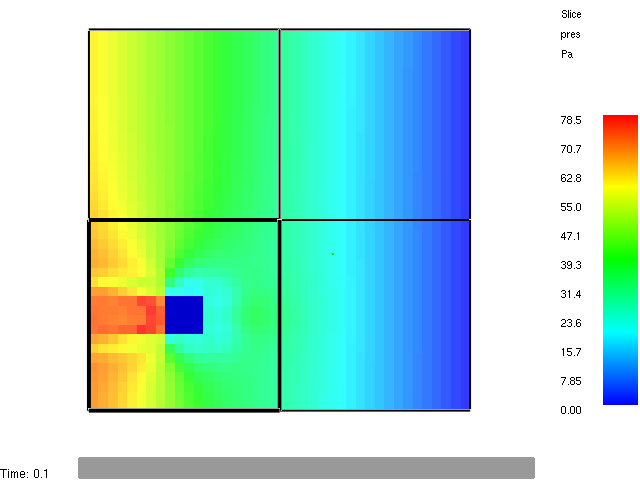
\includegraphics[width=8 cm]{\figPath/b4_le_0062.png}
\end{center}
\caption{Linear extrapolation  (LE) for Case 1}
\label{FIG_MGM_Grid}
\end{figure}


These both seems to be very similar.  But please note the displayed ranges (they are unchanged, as originally displayed by smokeview).
The display range for (LE) is a little closer to the single-mesh range. But I don't know if this matters.

\newpage
\subsubsection{Dancing\_eddies}
The usual pressure history plots for UGLMAT and USCARC (which both provide the same) against MGM with the (SM) and (LE) boundary settings.
\begin{figure}[H]
\begin{center}
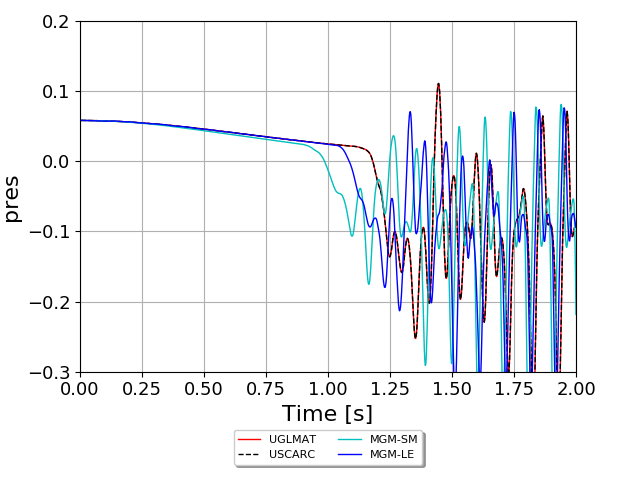
\includegraphics[width=10cm]{\figPath/dancing_eddies_pres.png}
\end{center}
\caption{Pressure histories of UGLMAT, USCARC, MGM-SM and MGM-LE for dancing\_eddies}
\label{FIG_MGM_de}
\end{figure}

And a more zoomed view here
\begin{figure}[H]
\begin{center}
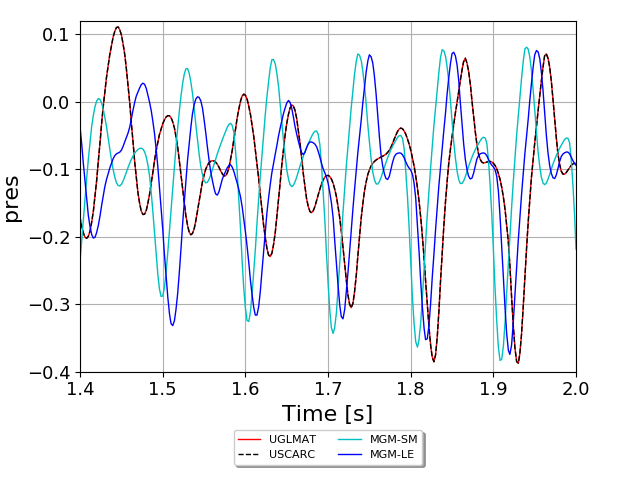
\includegraphics[width=10cm]{\figPath/dancing_eddies_pres2.png}
\end{center}
\caption{Zoomed pressure histories of UGLMAT, USCARC, MGM-SM and MGM-LE for dancing\_eddies}
\label{FIG_MGM_de}
\end{figure}

Here the differences seem to be more pronounced with a slight advantage for the linear extrapolation (the blue one). But they both don't fit the course of the
really unstructured solutions.

\newpage
\subsubsection{Pressure\_Iteration3d}
This is my pressure\_iteration3d case from the Pressure\_Solver directory (different and steadily changing ramp-based inflows from xmin, ymin and zmin)
with the pressure history for the green device position.

\begin{figure}[H]
\begin{center}
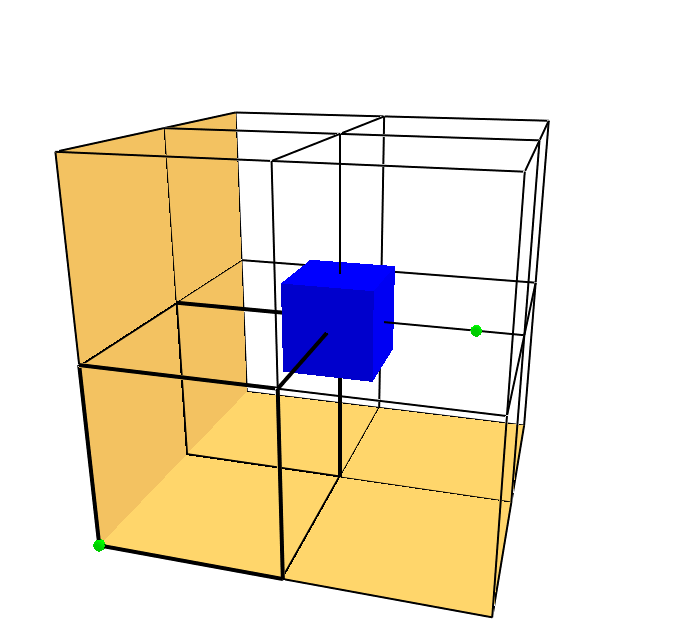
\includegraphics[width=5cm]{\figPath/pressure_iteration3d_uscarc_s0000.png}
\end{center}
\caption{pressure\_iteration3d case}
\label{FIG_MGM_pi}
\end{figure}

And here again are the plots for UGLMAT and USCARC (which again both provide the same) against MGM with the (SM) and (LE) boundary settings.
\begin{figure}[H]
\begin{center}
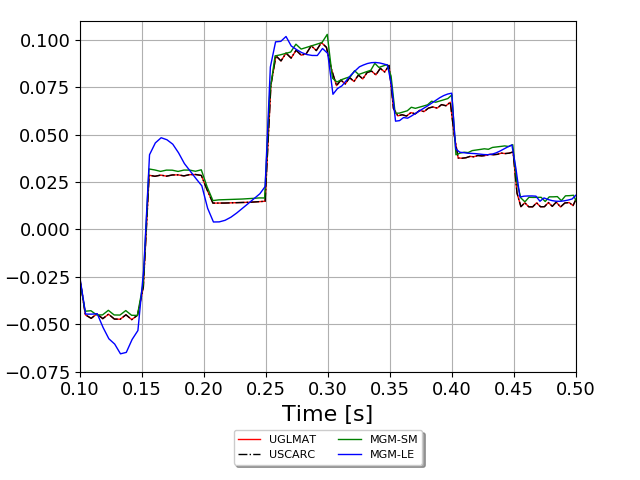
\includegraphics[width=12cm]{\figPath/pressure_iteration3d_pres.png}
\end{center}
\caption{Pressure histories of UGLMAT, USCARC, MGM-SM and MGM-LE for pressure\_iteration3d}
\label{FIG_MGM_pi}
\end{figure}

Here, the simple (SM) boundary condition seems to do the better job. But due to the steadily changing inflow conditions in this case this might be an issue of bad initial values for the extrapolation. 





% ---------  bibliography
\bibliographystyle{unsrt}
\bibliography{\bibPath/FDS_general,\bibPath/FDS_refs,\bibPath/FDS_mathcomp,bibliography}

%\addcontentsline{toc}{chapter}{References}

\end{document}

